\chapter*{Quantum and Spiritual Glossary}
\addcontentsline{toc}{chapter}{Quantum and Spiritual Glossary}
\markboth{Quantum and Spiritual Glossary}{Quantum and Spiritual Glossary}
\vspace{0.6cm}
\begin{center}
\nopagebreak
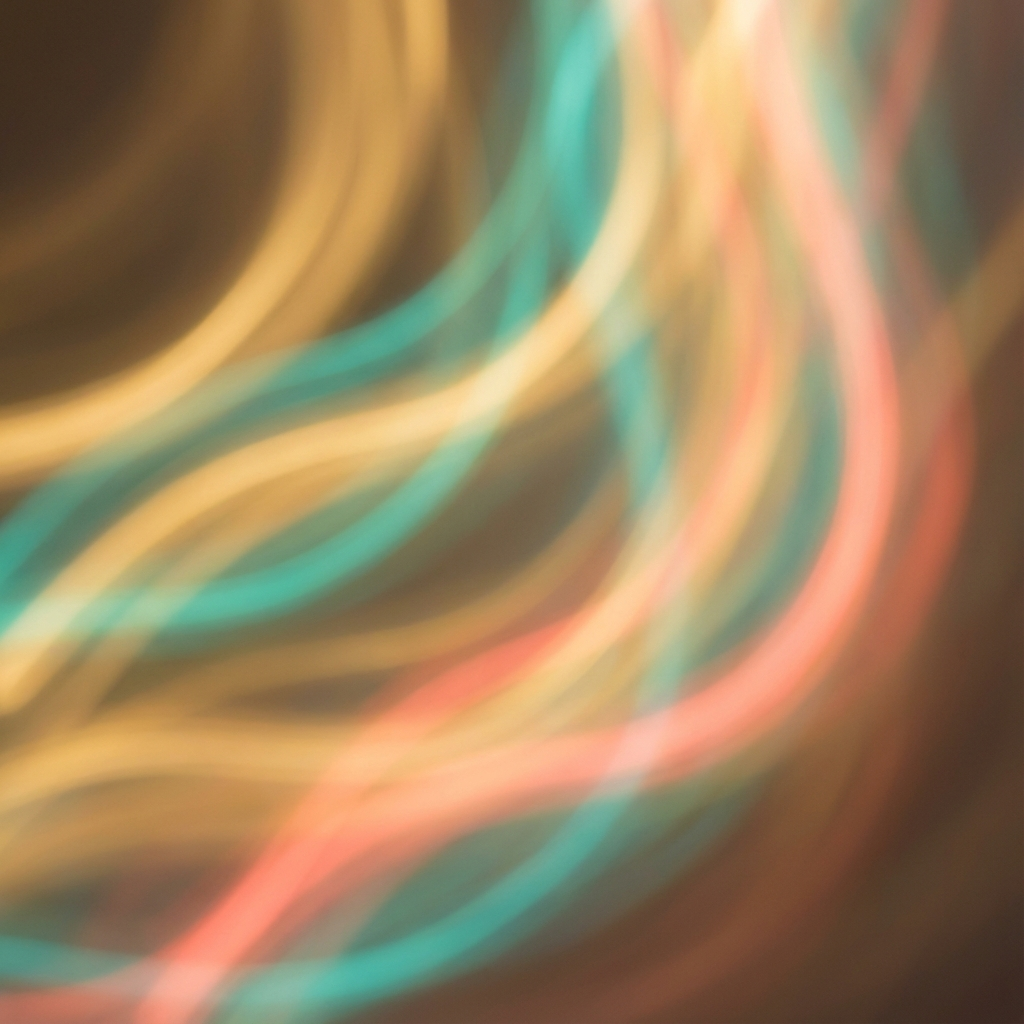
\includegraphics[width=0.75\textwidth,cfbox=gray!60 0.6pt 4pt]{vibration.png}\\
\vspace{4pt}
{\small\itshape The luminous bridge between quantum physics and Christ's wisdom.}
\end{center}

\vspace{0.6cm}
Para enriquecer tu experiencia y profundizar en los diálogos del Maestro, aquí tienes una guía de los conceptos clave donde la ciencia cuántica y la sabiduría interior se encuentran:


\vspace{0.4cm}
\begin{center}
\rule{0.35\textwidth}{0.4pt}
\end{center}
\vspace{0.4cm}


\subsection*{1. Abwoon (El Origen Cósmico)}
En la lengua aramea original en la que habló Jesús, \textit{Abwoon} no significa simplemente un patriarca humano, sino el \textbf{«Generador Cósmico de Luz y Aliento»}. Representa la Fuente omnipresente que crea, sostiene y expande continuamente todo el tejido del universo a través de la vibración del amor.


\vspace{0.4cm}
\begin{center}
\rule{0.35\textwidth}{0.4pt}
\end{center}
\vspace{0.4cm}


\subsection*{2. El Efecto Observador y la Fe}
En la física cuántica, una partícula permanece como una onda de infinitas posibilidades hasta que un observador interactúa con ella y «colapsa» esa probabilidad en una realidad física tangible. Jesús enseñó este mismo principio al decir: \textit{«Todo lo que pidáis en oración, creed que ya lo habéis recibido, y os vendrá»}. La fe es la certeza del observador consciente de que la Luz ya ha manifestado el resultado.


\vspace{0.4cm}
\begin{center}
\rule{0.35\textwidth}{0.4pt}
\end{center}
\vspace{0.4cm}


\subsection*{3. Entrelazamiento Cuántico y el Perdón}
El entrelazamiento cuántico demuestra que dos partículas conectadas continúan influyéndose mutuamente sin importar la distancia en el espacio-tiempo. Cuando guardamos resentimiento hacia alguien, quedamos energéticamente entrelazados con el dolor del pasado. El \textbf{perdón} es la única herramienta cuántica que corta ese lazo denso, liberando a ambas almas para que vuelvan a vibrar en sincronía con el presente.


\vspace{0.4cm}
\begin{center}
\rule{0.35\textwidth}{0.4pt}
\end{center}
\vspace{0.4cm}


\subsection*{4. Frecuencia Vibratoria y el Reino de los Cielos}
El universo entero está hecho de energía en constante oscilación. Las emociones como el miedo, la ira o la culpa vibran en frecuencias bajas y densas (la «gravedad» de la que habla Jesús). Las emociones como la gratitud, la paz y el amor incondicional vibran en frecuencias sutiles y elevadas. El \textbf{Reino de los Cielos} no es una ubicación geográfica futura, sino la frecuencia más alta del Ser: sintonizable aquí y ahora.


\vspace{0.4cm}
\begin{center}
\rule{0.35\textwidth}{0.4pt}
\end{center}
\vspace{0.4cm}


\subsection*{5. Coherencia Corazón-Mente}
Cuando los pensamientos de la mente y las emociones del corazón entran en resonancia armónica, el campo electromagnético que irradiamos se vuelve extraordinariamente potente y protector. Es lo que el Maestro definió como \textit{«pedir en mi nombre»}: alinearse con la misma frecuencia de la Presencia.